% 请在下方的大括号相应位置填写正确的节标题和标签,以及作者姓名
\section{使用\keyword{vi},\keyword{vim}创建文件}\label{sec:使用vi,vim创建文件}
\sectionAuthor{Jiaqi Z.}

% 请在下方的item内填写本节知识点
\begin{Abstract}
    \item 如何通过\code{vi},\code{vim}创建并保存文件
    \item 如何通过\code{vi},\code{vim}打开已有文件
\end{Abstract}

% 请在正文相应位置填写正确的小节标题(或小小节标题),同时将标签的“节标题”和“小节标题”改为实际内容

\subsection{通过\code{vi}创建文件}\label{subsec:使用vi,vim创建文件-通过vi创建文件}

从本节开始,这一章就要开始讨论\code{vi}和\code{vim}的操作方法。类似于使用\code{nano}编辑文件,在Linux当中通过\code{vi}(\code{vim})创建文件的方法是\code{vi <文件名>}或\code{vim <文件名>}。通常来说,使用\code{vi}创建文件后的界面如图\ref{fig:使用vi,vim创建文件-vim界面}所示。

\begin{figure}
    \centering
    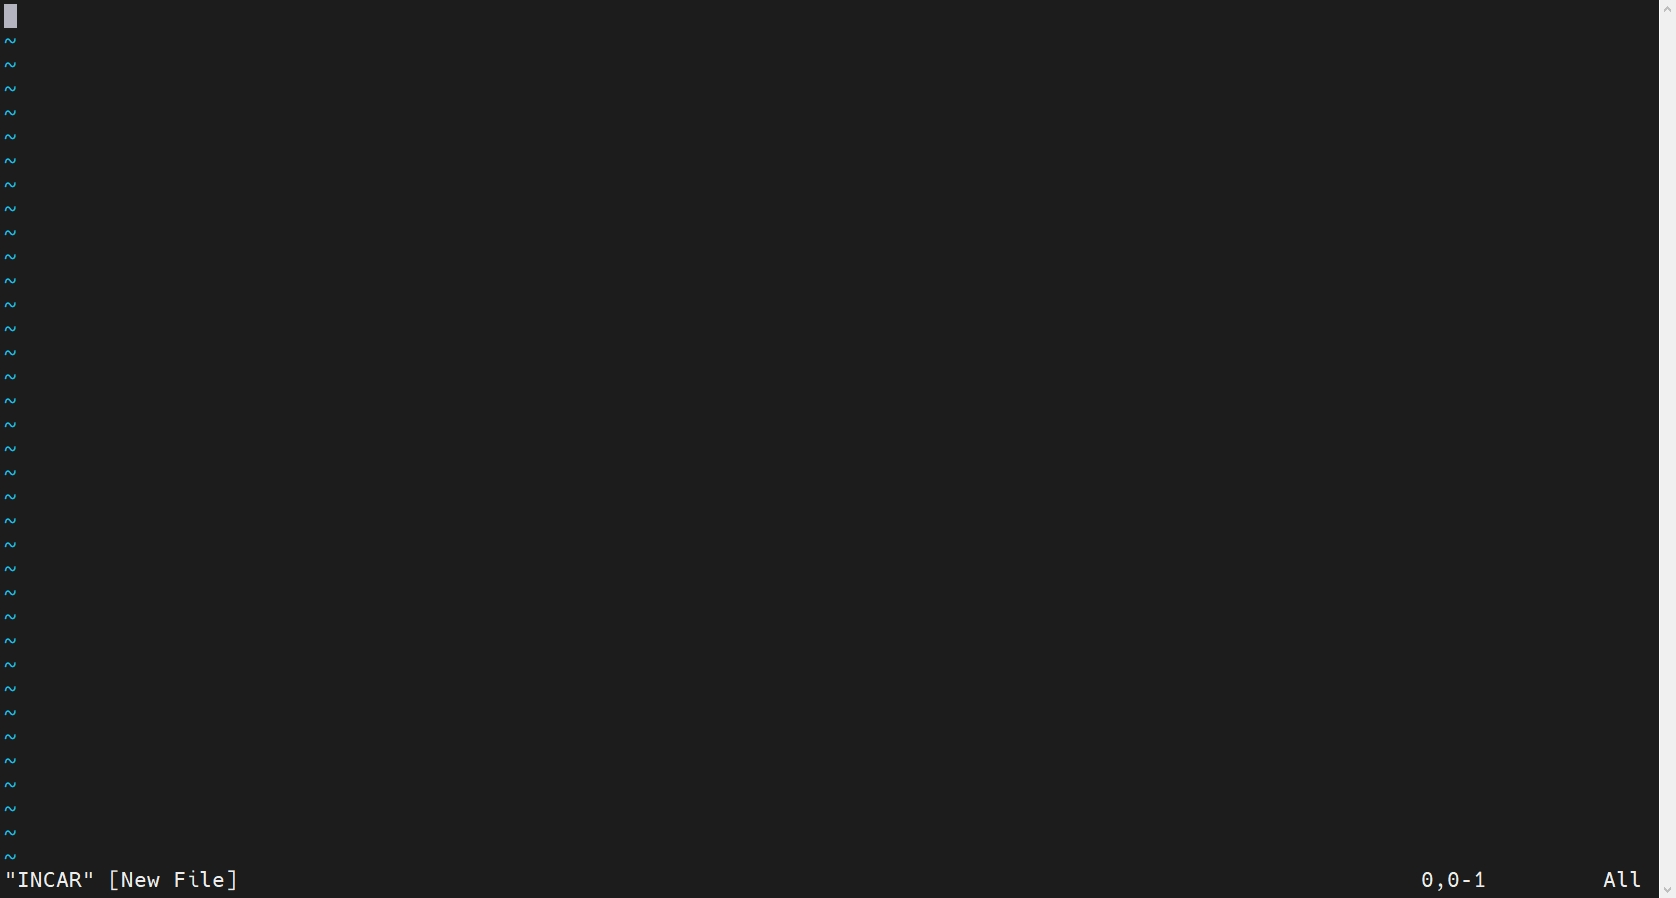
\includegraphics[width=1\linewidth]{Linux基础/文本编辑工具vi和vim/使用vi,vim创建文件/fig/vim界面.png}
    \caption{vim界面}
    \label{fig:使用vi,vim创建文件-vim界面}
\end{figure}

\begin{attention}
    仔细看图\ref{fig:使用vi,vim创建文件-vim界面}标题的话,可能会发现,明明说的是\code{vi}的创建文件,为什么显示的界面是\code{vim}呢?正如\ref{sec:使用nano简单创建文件}开头所说的那样,相比于vi,vim的功能更加强大。目前在很多操作系统当中,都是使用\code{vim}代替\code{vi}。因此,在本节标题中,我们使用\code{vi}和\code{vim}作为区分,在后面的讨论中,可能为了方便,我们使用\code{vi}代替\code{vim}(二者操作方法基本一致)。

    如果你确实想知道使用\code{vi}命令打开的是vim编辑器还是vi编辑器,可以使用\keyword{alias}命令,在输出中如果看到有\code{alias vi='vim'},那么说明实际上你所打开的是vim编辑器;如果没有,则意味着打开的是vi。此时如果希望打开vim编辑器,则需要使用命令\code{vim}代替\code{vi}。
\end{attention}

\subsection{vi编辑器的三种模式}\label{subsec:使用vi,vim创建文件-vi编辑器的三种模式}

与nano界面相比,vi界面显得更加“简洁”(没有了下方的菜单栏)。但是,如果你尝试着往里面输入内容的话,会发现往往不会是你想要的结果(也有可能“误打误撞”可以输入进去)。这是因为,在vi当中存在三种工作模式:

\subsubsection{普通模式}

当你使用\code{vi}命令打开编辑器后,则进入了编辑器的\emph{普通模式}。在这一模式下,你可以使用方向键移动光标,也可以进行删除、剪切、粘贴等简单操作。

一些简单的操作是使用\keywordin{vi}{x}键删除当前光标所在字符,使用\keywordin{vi}{dd}删除当前行(实际上是“剪切”),\keywordin{vi}{yy}复制当前行;使用\keywordin{vi}{p}(小写)将剪贴板内容粘贴到光标下方,\keywordin{vi}{P}大写表示粘贴到光标上方。\keywordin{vi}{u}表示撤销,\code{Ctrl+r}表示恢复撤销。

上面这些操作都是比较基础简单的,通常是用于对文件进行\emph{修改}的。而对于新创建的文件,则可以使用\keywordin{vi}{i}进入到“编辑模式”。同时,使用\keywordin{vi}{a}可以在光标下一个位置开始“编辑模式”,\keywordin{vi}{o}(小写字母)和\keywordin{vi}{O}(大写字母)分别表示在当前行下方和上方插入新的一行,并进入“编辑模式”

\subsubsection{编辑模式}

这是最熟悉的模式。可以在这一模式下如同正常文本编辑器一般进行编辑(例如,方向键移动光标,编辑字符,删除键等都是可用的)。除此之外,还有一些快捷键需要介绍一下\footnote{这些快捷键很多在Windows当中也有,但可能大多数人并不熟悉。}。

使用键盘上的\code{Home}键和\code{End}键可以将光标定位到行首和行尾;使用\code{Page Up}和\code{Page Down}可以上下翻页;使用\code{Insert}可以在“插入模式”和“替换模式”下切换。

在“编辑模式”下使用键盘上的\code{Esc}键可以返回到“普通模式”。

\subsubsection{命令行模式}

这一模式将会是最复杂的,许多vi的高级操作都是基于一系列的命令完成的。进入命令行模式的方法是\emph{在“普通模式”下输入键盘上的\code{:}}。

虽然大多数命令要在后面的章节提到它们,但一些必要的命令还是需要现在知道的--它们涉及到\emph{文件的保存}和\emph{编辑器的关闭}。例如,\keywordin{vi}{:w}表示保存文件,\keywordin{vi}{:q}表示关闭编辑器,\keywordin{vi}{:q!}表示强制退出(不保存),而\keywordin{vi}{:wq}表示保存后退出\footnote{它还有一个形式:\keywordin{vi}{:x}。}。

\subsection{通过\code{vi}打开已有文件}\label{subsec:使用vi,vim创建文件-通过vi打开已有文件}

类似于使用\code{nano <文件路径>}的方法,使用\code{vi}打开已有文件的方法是\code{vi <文件路径>}。与前面所介绍的内容一样,打开后的vi界面默认是“普通模式”,此时可以使用一些简单的方式(如\code{dd}删除整行等)对文件进行简单的编辑,或者可以使用“编辑模式”进行修改操作。

\begin{attention}
    在修改文件时,请确保是否有修改文件的权限。对于没有权限的文件进行修改,在退出时将会返回“'readonly' option is set (add ! to override)”的错误。

    正如错误中所说的那样,你可以使用\code{w!}的方式强行覆盖文件,但这始终是一种“下策”。
\end{attention}


\subsection{错误处理}\label{subsec:节标题-错误处理}
% 请在本节列出可能遇见的错误与解决方法

\subsubsection{E37: No write since last change (add ! to override) }

这表明你在\code{:q}退出时文件发生了修改。类似于WIndows操作系统下退出时询问是否保存一样,你需要选择是否保存你的编辑。如果保存,则需要先执行\code{:w}再\code{:q},或者直接执行\code{:wq};相对地,如果你不需要保存,则执行\code{:q!}强制退出。

\subsubsection{W10: Warning: Changing a readonly file}

这是一个警告信息,说明你正在编辑一个对你而言有权限限制的文件(大多数时候是“只读”文件,但对于某些“不可读”文件,如果强行编辑,可能也会引起该错误)。如果无视编辑并保存的话,通常会引发下面的错误:

\subsubsection{E45: 'readonly' option is set (add ! to override) }

这是正文最后所提到的错误,说明你编辑了一个有权限限制的文件。使用\code{:w!}可以强行覆盖保存文件,但这并不是一个正确的方法(至少是不推荐的方法)。

\subsubsection{ [Permission Denied] }

这是因为你在查看一个不可读的文件。当你尝试编辑时,则会引发上面的警告或错误。